\documentclass[11pt]{article}
\usepackage[utf8]{inputenc}
\usepackage{graphicx} 
\linespread{1.5}
\usepackage[bottom=2.5cm,top=2.5cm, margin=2.5cm]{geometry}
\usepackage[font=small,labelfont=bf]{caption}
\usepackage[round]{natbib} 
\bibliographystyle{plainnat}
\usepackage[T1]{fontenc}
\usepackage{imakeidx}
\makeindex[columns=3, title=Alphabetical Index, intoc]
\usepackage[hidelinks]{hyperref}
\usepackage{xcolor,soul,lipsum}
\newcommand{\myul}[2][black]{\setulcolor{#1}\ul{#2}\setulcolor{black}}


\topmargin=-0.5in

\usepackage{float}

\begin{document}
\begin{titlepage}
   \begin{center}
       \vspace*{5cm}

       \textbf{Can't Stand the Heat? An Analysis of the Thermal Sensitivity of Arthropods, How It Has Evolved \& Factors Influencing It}
       
       \vspace{2cm}
       \textbf{Author: Kate Griffin}
       
       \vspace*{2cm}
       \textbf{Supervisors: Dr. Samraat Pawar, Dr. Dimitris Kontopoulos, Dr. Paul Huxley,  Dr. Lauren Cator}
       
       \vspace{2cm}
       August 2022
            
       \vspace{4cm}
       \small
       A thesis submitted in partial fulfilment of the requirements for the degree of Master of Science at Imperial College London.
       \linebreak
       \small
       Submitted for the MSc in Computation Methods in Ecology \& Evolution.

       \vfill
            
  \end{center}
\end{titlepage}
\clearpage

\vspace{10cm}

\paragraph{Declaration}\mbox{}\\
I declare that I am the sole author of this thesis. For this project, the data was collected from fifty-two studies, which are given in Table S2 in the supplementary information. The collection, processing, cleaning and digitisation of the data used in this project was a collaborative effort between myself, Dr. Paul Huxley and Tianle Shao. The data was digitised under the VecTraits framework, developed by my supervisor Dr. Samraat Pawar. The approach for fitting the Sharpe-Schoolfield model used in this project was developed by my co-supervisor, Dr. Dimitris Kontopoulos. I developed the regression models used in this analysis under the guidance of my co-supervisor Dr. Dimitris Kontopoulos. I developed the methodology for this project under the guidance of my supervisor, Dr. Samraat Pawar, and my co-supervisors, Dr. Dimitris Kontopolous, Dr. Paul Huxley and Dr. Lauren Cator.

\vspace{2cm}Word Count: 5,032

\clearpage
\tableofcontents
\clearpage

\begin{flushleft}

\section{Abstract}
Arthropods play an important role in food security, maintaining ecosystem services, nutrient cycling, decomposition and more. Therefore, it is important to understand how they adapt to changing temperatures, particularly in light of climate change. The effect of temperature on the performance of a given fitness-related trait can be described by a thermal performance curve (TPC). Thermal sensitivity \emph{($E$)}, or “activation energy” controls the steepness of the rising portion of a thermal performance curve up to its maximum, and describes how the performance of a given biological trait responds to changes in temperature. The Metabolic Theory of Ecology expects that \emph{$E$} is constant across all traits and taxa, and falls within a range between 0.6-0.7 eV. This is also referred to as the Universal Temperature Dependence (UTD). Empirical evidence against the UTD in recent years has sparked debate about its validity. Developing a comprehensive understanding of how thermal sensitivity has evolved in arthropods can provide a basis for predicting how such species may respond to changes in global temperatures.
The main aims of this analysis are to (i) estimate the activation energy of arthropods to determine if thermal sensitivity is conserved through evolutionary time, (ii) examine whether thermal sensitivity in arthropods adheres to the UTD theory and (iii) analyse the effect of body size, latitude and the interaction of body size and latitude on the thermal sensitivity of arthropods. The results of this analysis show (i) no evidence that thermal sensitivity is conserved through evolutionary time, and may be affected by convergence, and (ii) thermal sensitivity of arthropods does not adhere to the expectations of the UTD, and falls outside of the 0.6 to 0.7 range. This may be the result of multiple factors affecting trait performance, the effect of multiple enzymes on biochemical kinetics, variation in species and ecological niches or experimental bias. (iii) Latitude, size and the interaction of latitude and size were all found to have a significant effect on thermal sensitivity. The relationship between \emph{E} and all three variables were found to be linear. Overall, these results indicate that the thermal sensitivity of arthropods is affected by many factors, such as latitude and body size. Developing a better understanding of the physiological mechanisms underpinning the thermal performance of biological traits may help protect arthropod species vulnerable to climate change.

\clearpage

\section{Introduction}
Arthropods are the most species-rich phylum in the animal kingdom, dominating virtually every ecosystem and surpassing all other taxonomic groups in terms of biomass, species richness and ecological function \citep{baillie2012spineless, doi/10.2779/27353}. They play a pivotal role in food security, maintenance and structure of ecosystems, nutrient cycling and pest control. Some are also used as valuable climatic indicators \citep{baillie2012spineless}. Globally, 40\% of insect species are threatened with extinction \citep{sanchez2019worldwide}. This is primarily due to climate change, habitat loss and fragmentation, invasive species and use of pesticides and insecticides \citep{borrell2012one,doi/10.2779/27353,sanchez2021indirect,simaika2018insect}. The global biomass of insects falls by 2.5\% each year \citep{sanchez2019worldwide}. Despite this decline, little priority has been given to conserving insect populations \citep{baillie2012spineless,doi/10.2779/27353,donaldson2016taxonomic,prather2013invertebrates,simaika2018insect}. For example, the EU Birds and Habitat directive grants protective status to 64.8\% of vertebrate species, but only 0.1\% of the invertebrate species in Europe. The IUCN Red List has assessed and categorised 71\% of all vertebrate species, compared to only 2\% of invertebrate species \citep{karam2020conservation}. There is also a considerable lack of data, expertise and taxonomic coverage of arthropods \citep{donaldson2016taxonomic,karam2020conservation,simaika2018insect}. A gap in public knowledge of the value which arthropods have in maintaining ecosystem health, as well as public support being granted to more “charismatic” animals, may be factors into this relative lack of conservation focus \citep{baillie2012spineless,doi/10.2779/27353}.
\linebreak

The United Nations’ Intergovernmental Science-Policy Platform on Biodiversity and Ecosystem Services (IPBES) has posited that the Earth’s ecosystem health has declined at an unprecedented rate \citep{diaz2019summary}. According to reports, global average temperatures may rise up to 5℃ by the end of the 21st century \citep{tollefson2020hot}. As arthropods are ectothermic, they are sensitive to shifting patterns in temperature \citep{doi:10.1073/pnas.2002543117}. One reason for this is due to the effect of temperature on metabolic processes \citep{schulte2015effects}. Body size plays an important role in these processes, as the Metabolic Theory of Ecology (MTE) states that metabolic trait performance and body size have a negative correlation across various taxonomic groups (i.e., the smaller an organism's mass, the higher its metabolic rate is likely to be) \citep{frazier2006thermodynamics}. Latitude also significantly affects the metabolism of ectotherms \citep{delong2018habitat} as temperature is directly affected by latitude (i.e., lower latitudes tend to have higher temperatures and temperature tends to decrease with distance from the equator). Studies have found that selection for “thermal generalists” (i.e., low thermal sensitivity) tend to be high in low to intermediate latitudes \citep{kontopoulos2020adaptive}. Understanding how arthropod fitness responds to changes in temperature may allow for (i) more effective safeguarding of natural resources and (ii) implementation of environmental policies which mitigate negative impact on ecosystems \citep{smith2019community}. 
\linebreak 

The effect of temperature on the performance of a given fitness-related trait can be described by a thermal performance curve (TPC). TPCs for biological rate traits (e.g., metabolic rate and respiration rate) usually take on the shape of a negatively skewed unimodal curve (Fig. 1) \citep{angilletta2006estimating,kontopoulos2020adaptive,schulte2015effects}. The curve rapidly increases until it reaches its maximum (i.e, temperature of peak performance, \emph{$T_{pk}$}). After it reaches its peak, it decreases exponentially. The rising portion of the TPC is controlled by the thermal sensitivity, \emph{$E$} (eV) or “activation energy", of the organism \citep{kontopoulos2020adaptive}. As \emph{$T_{pk}$} tends to be higher than the mean environmental temperature, $E$ represents thermal sensitivity within its typically experienced temperature range. The declining portion of curve represents \emph{$E_D$} (eV), which describes how steeply the TPC falls. \emph{$E_D$} is generally steeper than \emph{$E$} \citep{kontopoulos2020adaptive}. The increase in trait performance up to \emph{$T_{pk}$} may be mechanistically described using the Boltzmann-Arrhenius equation (Eqn. 1):
\begin{equation}
B_0 \times e[\frac{-E}{k}(\frac{1}{T} - \frac{1}{T_{ref}})]
\label{eq:1}
\end{equation}
\newline
\emph{T} is temperature (in K). \emph{B} represents the value of the trait being modelled. \emph{$B_0$} is a normalisation constant which represents the trait value at a reference temperature and includes the effect of body or cell size (\emph{$T_{ref}$}). The Boltzmann constant ($8.617.1 ^{-5} eV \times K^{-1}$) is represented as \emph{k}. 
Early metabolic theory states that \emph{$E$} is practically constant across all traits and species, and falls within a range of 0.6-0.7 eV (i.e., a Universal Temperature Dependence, or "UTD", exists) \citep{gillooly2001effects,clarke2004there,pawar2016real,irlich2009insect}. This idea is based on the putative mean activation energy of respiration ($\approx$ 0.65 eV) \citep{kontopoulos2020adaptive,white2012information}. The UTD has been disputed in recent years, with newer evidence suggesting that \emph{E} may not conform to the 0.6 - 0.7 eV range expected by the Metabolic Theory of Ecology \citep{pawar2016real,irlich2009insect,kontopoulos2020adaptive,clarke2004there,white2012information}. It has been argued that the UTD theory is too simplistic to describe all biological variation, but rather represents a useful baseline for which variation in biological systems may be examined \citep{white2012information}. MTE states that the effect of temperature on trait performance reflects the thermal sensitivity of the kinetics of a single rate limiting enzyme \citep{kontopoulos2020adaptive,clarke2004there}. However, it may be argued that the Boltzmann-Arrhenius model fails to describe TPCs which result from interactions of multiple factors and not just that of temperature on biochemical kinetics \citep{kontopoulos2020adaptive,white2012information,pawar2016real}. 
\newline
\newline
\begin{figure}[h]
    \centering
    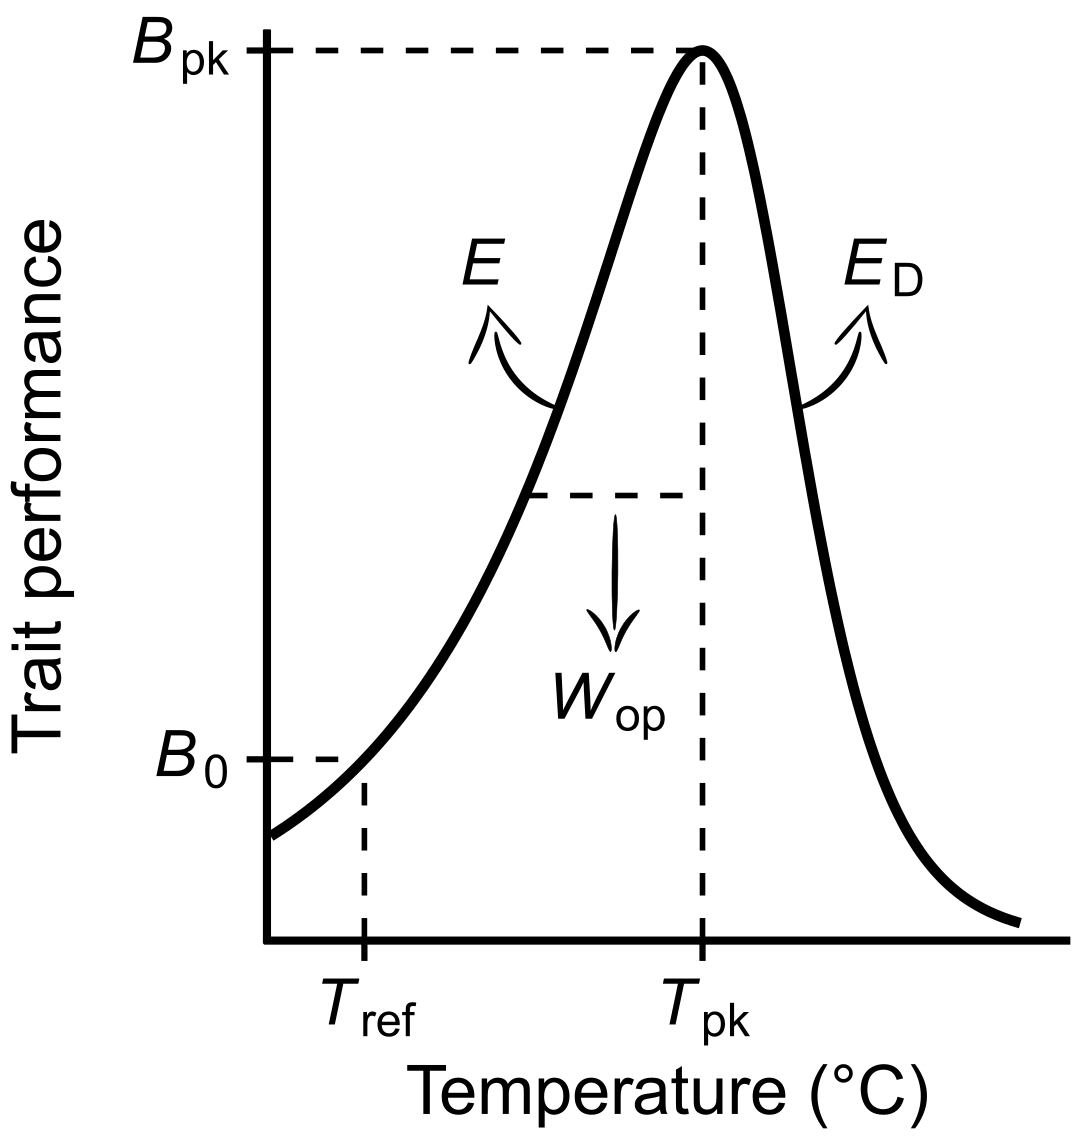
\includegraphics[width=3.8in]{example_tpc.png}
    \caption{\label{fig:1} Example of a thermal performance curve \citep{kontopoulos2020adaptive}. \emph{E} (eV) is thermal sensitivity of the trait at the rising portion of the TPC. \emph{T} is temperature in K. \emph{$T_{pk}$} is the temperature of peak performance. \emph{$E_D$} (eV) describes how the TPC decreases after \emph{$T_{pk}$}. \emph{B} is the value of a given biological trait and \emph{$B_0$} is a normalisation constant which gives a trait value at a reference temperature, \emph{$T_{ref}$}. \emph{$B_{pk}$} is trait value at peak performance. \emph{$W_{op}$} is the operational niche width of the TPC}.
\end{figure}
\newline

Deviations from the UTD may be explained by looking at how thermal sensitivity has evolved, which we can investigate by calculating its phylogenetic signal (i.e., "phylogenetic heritability"). \citep{kontopoulos2020adaptive}. Phylogenetic signal can be defined as the tendency of related species to resemble each other more so than species randomly drawn from the same phylogenetic tree \citep{munkemuller2012measure}. It can provide valuable insights into how variation of thermal sensitivity of traits has evolved across different taxa. Phylogenetic signal can be measured using Pagel's lambda ($\lambda$), which is a scaling parameter between 0-1 \citep{pagel1999inferring}. When phylogenetic signal is equal to 1, then evolution of said trait is adhering to to Brownian motion (i.e., a random walk over tree space through evolutionary time) \citep{molina2017revisiting,munkemuller2012measure,pagel1999inferring}. A phylogenetic signal of 0 indicates that traits have evolved independently of phylogeny and, therefore, close relatives are no more similar to each other than distant relatives \citep{molina2017revisiting}. Values in between 0 and 1 demonstrate deviations from Brownian motion, possibly as a result of convergence \citep{kontopoulos2018use}.
\linebreak

The main aims of this analysis are:
\begin{itemize}
    \item To estimate the thermal sensitivity of a number of arthropod species and to determine whether thermal sensitivity in arthropods is conserved through evolutionary time.
    \item Determine if thermal sensitivity of arthropods falls within a range of 0.6 to 0.7 eV, and thus conforms to a central expectation of traditional MTE.
    \item Analyse the effect of (i) body size (ii) latitude and (iii) the interaction between body size and latitude on the thermal sensitivity of arthropods.
\end{itemize}

I hypothesise that (1) thermal sensitivity is, to some degree, phylogenetically heritable and (2) the thermal sensitivity of arthropods does not adhere to the expectations of the Universal Temperature Dependence.
\clearpage

\section{Methods}
\subsection{Data collection}
The data for this analysis was collected from eighty-two papers which provided laboratory measurements of metabolic rate of arthropods across constant temperatures (Table S2) using the VecTraits framework \citep{samraat_pawar_2016_57356}. Figures were digitized using WebPlotDigitizer v4.5. Analyzing digitised data from the literature can allow for more informative comparisons and, therefore, more confidence in the results. Life stage and sex of individuals were noted. Measurements for body mass (/g of mean wet mass), location and experimental conditions were recorded when provided. When individual body mass was not provided, estimates for this trait were sourced from other studies on the same species. A unique ID was given for each TPC, subsetting the data by species, population, life stage and metric for metabolic rate. While metabolic rate measurements and units vary substantially across studies, this is not an issue when estimating \emph{E} as it is calculated from the gradient of the TPC. The resulting dataset contained metabolic measurements from 142 species from 48 families. 
\linebreak

\subsection{TPC model Fitting}
To obtain estimates of thermal sensitivity (\emph{E}), thermal performance curves (TPCs) were fitted to the data using the Sharpe-Schoolfield equation. This model extends the Boltzmann-Arrhenius equation (Eqn. \ref{eq:1})  to include trait performance in the declining portion of the unimodal curve (i.e., \emph{$E_D$}), after the TPC reaches its peak (\emph{$T_{pk}$}). The method for fitting the Sharpe-Schoolfield model followed the same approach as Kontopoulos et al. (2020b; 2020a). This method used a 4-parameter variant of the Sharpe-Schoolfield model. The four parameter estimates obtained are $E$ (thermal sensitivity in the rising portion of the TPC), \emph{$T_{pk}$} (temperature of peak performance), \emph{$E_D$} (thermal sensitivity in the declining portion of the TPC) and \emph{$B_0$}, (a normalisation constant which factors in body size and gives the trait value at a reference temperature (\emph{$T_{ref}$})). 
\linebreak

Subsets with less than four observations for metabolic rate were filtered out before running the TPC analysis. Subsets with less than three unique temperature points were also filtered out. After initial filtering, sixty-three species remained. The starting value for \emph{$B_0$} was set as the minimum trait measurement at the rise of the TPC. The starting value of \emph{$T_{pk}$} was set to the temperature at which the trait reaches its maximum value. Starting values for \emph{$E$} were set as the slope of the regression for each subset where measurements were given before the thermal optimum. Otherwise, the starting value for \emph{$E$} was set to an estimate of 0.6 eV. For subsets which contained measurements after the thermal optimum, a starting value for \emph{$E_D$} was given as the slope of the regression. \emph{$E_D$} for subsets which did not contain this data was set to 3 eV. \emph{$R^2$} was calculated and TPCs with \emph{$R^2$} values less than 0.5 were excluded from the analysis. TPCs with less than three data points up to the peak were also removed. Any TPCs with values for \emph{$E$} above 2.5 eV were also filtered out. After fitting the Sharpe-Schoolfield model to each subset and final filtering, parameter estimates were obtained for fifty-five species.
\linebreak

\subsection{Phylogenetic reconstruction}
The Open Tree of Life topology \citep{hinchliff2015synthesis} for the resulting fifty-five species was obtained using the rotl R package (version 3.0.12).\citep{michonneau2016rotl}. The topology was manually examined to ensure there were no incorrect matches. A time tree was created using timetree.org based on the species from the Open Tree of Life topology. This was done using the “congrufication" approach, which uses a “reference tree" (scaled to time), to time calibrate a “target" tree (not scaled to time) \citep{eastman2013congruification}. Divergence times were transferred from the time tree to the OTL topology. Any nodes which were incompatible between the two trees, or those without any age information, were scaled using the treePL program \citep{smith2012treepl}. The tree was pruned using the keep.tip function from the phytools package in R (version 1.0 -3). Phylogenetic trees were created using phylotool’s dotTree function. 
\linebreak

Phylogenetic signal of \emph{E} was calculated using phylotool’s phylosig function. Phylosig takes values for a single continuously distributed trait and a phylogenetic tree in phylo format and returns estimates, as well as hypothesis tests, for significant phylogenetic signal. Pagel’s lambda ($\lambda$) was used to determine the phylogenetic relationship between species. Lambda is a measure of phylogenetic signal whereby the degree to which a shared evolutionary history between taxa has driven trait distributions at the tree’s tips. It estimates phylogenetic signal using maximum likelihood. Pagel’s  $\lambda$ assumes a classic Brownian motion evolutionary model (i.e. random walk over evolutionary time) \citep{molina2017revisiting,munkemuller2012measure,pagel1999inferring}. The variance in the distribution of trait values is proportional to the tree’s branch lengths \citep{munkemuller2012measure}. Values of lambda range between 0 to 1. When lambda is equal to 0, no phylogenetic signal can be inferred; therefore, the trait has evolved independently. Values close to 1 indicate trait evolution according to Brownian Motion \citep{molina2017revisiting,munkemuller2012measure}. Phylosig was run 1000 times on the \emph{$E$} estimates and the pruned species tree, each time saving the values for  $\lambda$ estimate, log likelihood and \emph{p}-value. Uncertainty around \emph{E} estimates was also accounted for to reduce bias towards lower $\lambda$ estimates. The $\lambda$ value corresponding to the highest log likelihood value was selected (Table \ref{table:1}).
\linebreak

\subsection{Regression analysis}
The data were fitted to weighted linear and polynomial regression models in order to predict how \emph{$E$} responds to changes in (i) latitude (ii) body mass and (iii) the interaction between latitude and body mass. Weights were set to $1/SE^2$ for each model (where SE is the standard error of \emph{$E$}). Predictions for each linear model were calculated by adding the intercept and slope given by the model's coefficients and multiplying by a sequence of maximum and minimum values for each variable (i.e., $intercept + (slope \times sequence)$). For each polynomial model, \emph{$E$} was predicted by multiplying a sequence of the maximum and minimum values for each variable by (i) the slope of the first degree coefficient and (ii) the slope of the second degree coefficient of the regressions and adding these values to the intercept (i.e., $intercept + (slope 1 \times sequence) + (slope 2 \times sequence)$). The predictions were plotted and examined. The residuals for each model were also calculated in R and plotted against fitted values (Fig. S5-S10). Phylogenetic signal was estimated from the residuals of these models to determine if the relationship between \emph{E} and latitude, size and the interaction between latitude and size is affected by phylogeny. Evidence for phylogenetic signal in the residuals of the regressions would indicate a need to correct them for phylogeny to get unbiased estimates of coefficients. Estimates for $\lambda$ were calculated by running phylosig on the residuals of each model and the pruned species tree 1000 times. As before,  values for  $\lambda$ estimate, log likelihood and \emph{p}-value were saved. The  $\lambda$  estimates corresponding to the highest log likelihood values for each model were selected and compared (Table \ref{table:1}). 
\linebreak

\paragraph{(i) $\emph{E} \sim $ Latitude }\mbox{}\\
A linear model was fitted with absolute latitude as the explanatory variable and \emph{$E$} as the response variable. The slope and intercept from the model’s coefficients were used to calculate the model’s predictions of \emph{$E$} for absolute latitudes between -55 to 80 by adding the intercept to the slope multiplied by absolute latitude (i.e., $intercept + slope \times |latitude|$). For the linear regression, values for absolute latitude were chosen. This is because specifying a linear model to the actual latitude values would assume that \emph{E} should increase/decrease from pole to pole (rather than increasing or decreasing from the equator to the North or South pole).
\linebreak

A second order polynomial regression model was also fitted to \emph{$E$} for latitudes between -55 to 80. As polynomial regression does not assume a linear relationship, then both negative and positive latitude values could be used rather than absolute latitude. Predicted values were calculated by multiplying the gradients of both the (i) first order and (ii) second order coefficient of the polynomial by latitude and adding these values with the intercept  (i.e., $intercept + (slope 1 \times latitude) + (slope 2 \times latitude$)). The model predictions were plotted on a graph along with observations for \emph{$E$} at latitudes between -55 to 80.  
\linebreak

\paragraph{(ii) $\emph{E} \sim$ Body Mass} \mbox{}\\
A linear regression model was used to analyze the relationship between activation energy and the log of the mean body mass for each species. Values for body mass given in dry mass were multiplied by three to estimate the wet mass. The fitted values were calculated by adding the intercept to the gradient multiplied by the log of mean body mass, which ranged from -9 to 3 (i.e., $intercept + slope \times log(mass)$). 
A second order polynomial regression model was also fitted to predict \emph{$E$} in response to changes in body mass. The fitted values were calculated by multiplying the slopes of the first and second order coefficient of the polynomial by the log of the mean body mass and adding these values to the intercept (i.e., $intercept + (slope1 \times mass) + (slope2 \times mass))$. The models’ predictions were plotted on a graph along with observations for \emph{$E$} at logged body masses between -9 to 3. 
\linebreak

\paragraph{(iii) $\emph{E} \sim$ Latitude $\times$ Body Mass}\mbox{}\\
Lastly, regression models were fitted to predict how \emph{$E$} responds to an interaction between body size and latitude (i.e., does \emph{$E$} vary among individuals of the same body mass at different latitudes or individuals of different body masses in the same latitudes). The linear model was fit using absolute latitude multiplied by the log of mean body mass as the explanatory variable. Predicted values were calculated by multiplying the slope by a sequence between -400 to 200 and adding the intercept (i.e., $intercept + slope \times (|latitude| \times log(mass)))$.
A second order polynomial was fitted and predicted $E$ values were calculated by multiplying the slopes of the first and second order coefficient of the polynomial by the log of mean body mass $\times$ latitude and adding these values to the intercept, i.e., $intercept + (slope 1 \times (mass \times latitude)) + (slope 2 \times (mass \times latitude))$. The models were plotted on a graph along with observations for E. 
\newpage

\section{Results}
\subsection{Phylogenetic reconstruction}
\paragraph{Estimating thermal sensitivity}\mbox{}\\
Values of thermal sensitivity (\emph{E}) for fifty-five species from twenty-eight families were estimated (Fig. \ref{fig:2}) using the Sharpe-Schoolfield equation (Eqn. 1). Species were subsetted by (1) life stage (2) the metric used for metabolic rate (i.e., resting metabolic rate or active metabolic rate). Eight species were filtered out from the analysis as they did not meet the given criteria (see methods). The means and medians were compared. No significant difference was found between different life stages or different measures for metabolic rate (Fig. S1-S4). A Shapiro-Wilk test was run using the shapiro.test function in R. This test checks for normality in the distribution of of a continuous variable \citep{SHAPIRO1965}. The distribution for \emph{E} was shown to deviate from a normal distribution (with a \emph{p}-value $<$ 0.05). Therefore, bootstrapping was chosen as the method for calculating the 95\% confidence interval for the \emph{$E$} distribution. \emph{E} was resampled 1000 times using the boot package in R. The mean value for $E$ across all species was calculated at $\approx$ 0.92 eV and the median $\approx$ 0.77 eV.
\begin{figure}[h] 
    \centering
    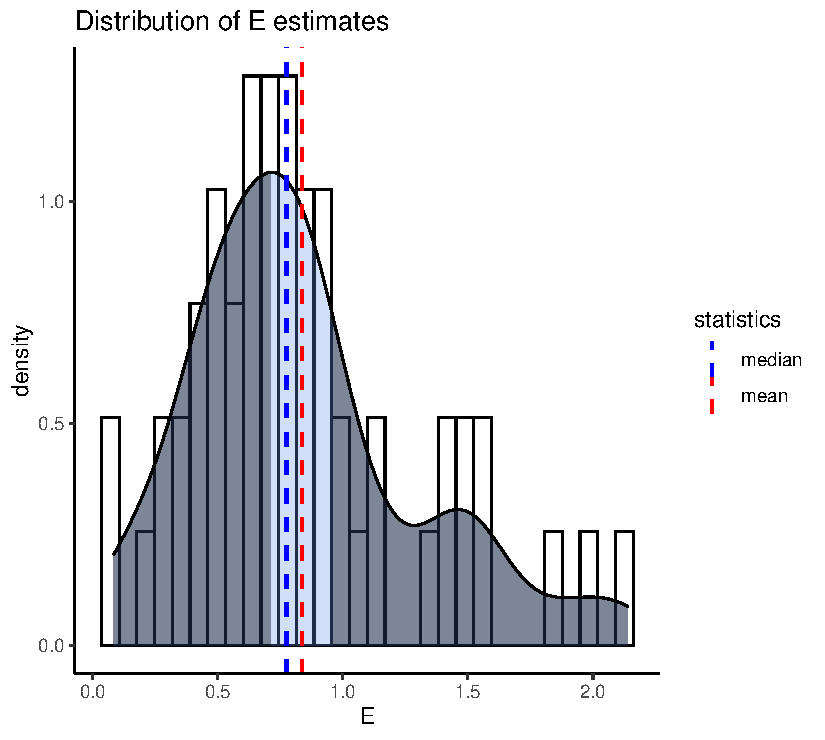
\includegraphics[width=3.45in]{E_DIST.pdf}
    \caption{\label{fig:2} Distribution of \emph{$E$} estimates for 55 species from 28 families. The dark shaded area represents the upper and lower bounds of the $95\%$ confidence interval. The mean is represented by the broken red line, and the median is represented by the broken blue line. The mean value of \emph{E} across all species was calculated at 0.92 eV, falling outside of the expected range of 0.6 to 0.7. These results indicate that \emph{E} does not adhere to the expectations of the UTD.}
\end{figure}
\newpage

\paragraph{Estimating phlogenetic signal}\mbox{}\\
Lambda ($\lambda$) was calculated for all species using (i) the estimated \emph{$E$} values calculated by the Sharpe-Schoolfield model, and then again using (ii) the residuals of the regressions of \emph{E} $\sim$ latitude, \emph{E} $\sim$ size and \emph{E} $\sim$ latitude  $\times$ size (Table \ref{table:1}). Log Likelihood estimates for each fit are also provided in (Table \ref{table:1}). All $\lambda$ values were less than 1 and more than 0, suggesting deviations from Brownian Motion. The mean and median were calculated for the $\lambda$ estimate of \emph{E} at $\approx$ 0.5, and the 95\% confidence interval was also calculated (Fig. \ref{fig:3}). The wide confidence intervals of $\lambda$ estimate for \emph{E} suggest that the data are not informative enough to allow for a conclusion to be drawn on the strength of the phylogenetic signal of \emph{E} (Fig. \ref{fig:3})
\linebreak

\begin{table}[!htbp]
\centering
\small
 \begin{tabular} {||p{3.7cm}p{2.9cm}p{2.5cm}p{3.2cm}||}
 \hline
 Variable & Model Type & $\lambda$ (ML estimate) & Max. Log Likelihood \\ [1.5ex] 
 \hline\hline
 Thermal sensitivity (\emph{E}) & Sharpe-Schoolfield & 0.0005 & -30.0758 \\
 \emph{E} $\sim$ Latitude & Linear & $4.8135e-05$ & -15.6951 \\ 
  & Polynomial & 0.4025 & -14.5554 \\
 \emph{E} $\sim$ Size & Linear & $6.6393e-05$ & -15.5608 \\
  & Polynomial & $7.3889e-05$ & -15.7037 \\
 \emph{E} $\sim$ Latitude $\times$ size & Linear & 0.5705 & -6.5785 \\ 
  & Polynomial &  0.7354 & -17.0752 \\ [2ex] 
 \hline
 \end{tabular}
 \caption{\label{table:1} Model estimates for phylogenetic signal ($\lambda$) of (i) \emph{$E$} estimates and (ii) the residuals of the regression of \emph{E} against latitude, size (mean body mass) and latitude $\times$ size. Values for $\lambda$ all lie between 0 and 1 demonstrate deviations from Brownian motion. These results may be due to convergence, or possibly high error in the data}.
\end{table}

\begin{figure}[!htbp]
    \centering
    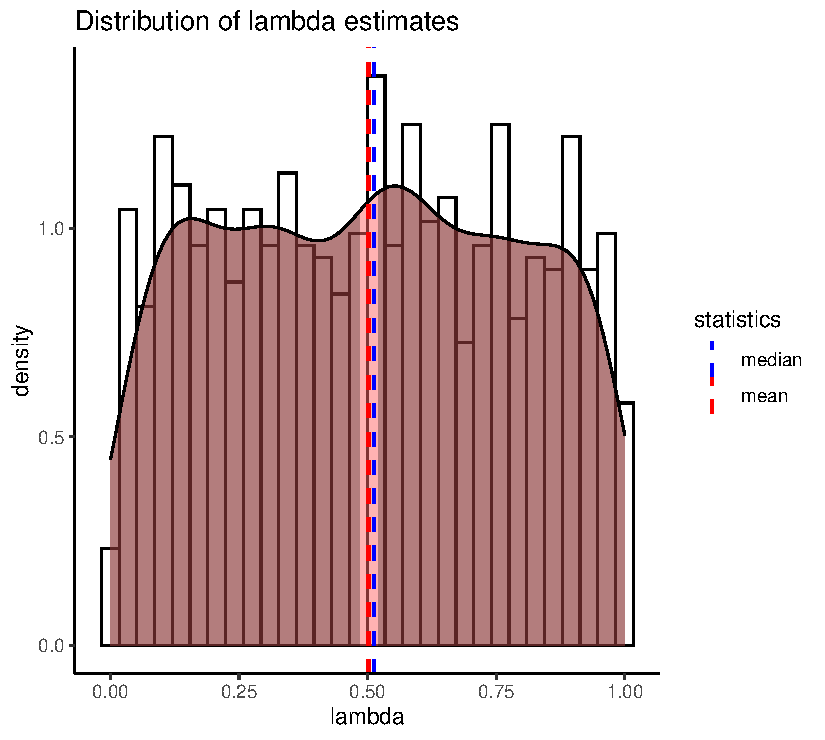
\includegraphics[width=5in]{lambda_dist.pdf}
    \caption{\label{fig:3} Distribution of $\lambda$ estimates sampled from 55 species from 28 families. The dark shaded area represents the upper and lower bounds of the $95\%$ confidence interval. The mean is represented by the broken red line, and the median is represented by the broken blue line. The width confidence intervals indicate that the strength of $\lambda$ cannot be determined possibly as a result of high error in the data.}.
\end{figure}
\newpage

\paragraph{Constructing phylogeny}\mbox{}\\
A phylogenetic dot tree was constructed using the \emph{$E$} estimates and a time calibrated topology. Varying sized dots/circles represent different tip values for \emph{$E$}. No conclusion could be drawn about the phylogenetic heritability of \emph{$E$} from this data (Fig. \ref{fig:4}).
\linebreak

\begin{figure}[!htbp]
    \centering
    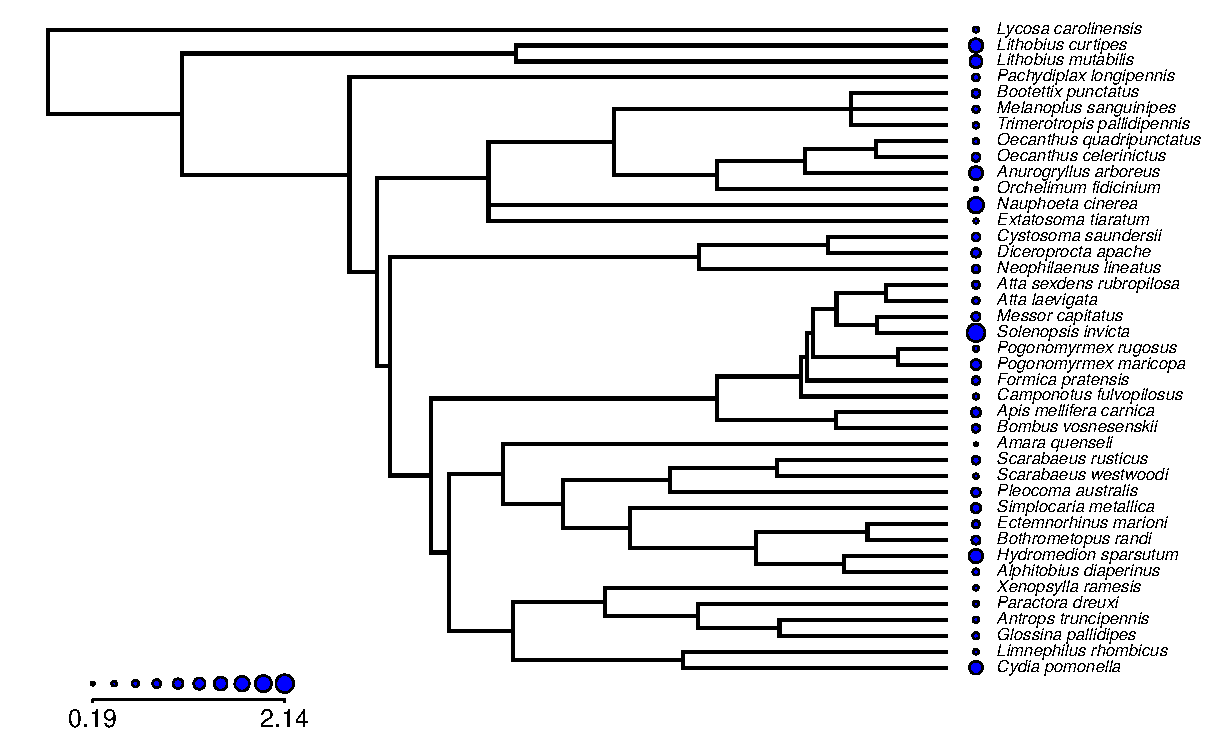
\includegraphics[width=6in]{dottree.pdf}
    \caption{\label{fig:4} Dot tree plot demonstrating the phylogenetic relationship of sample species and their corresponding estimated values for \emph{$E$}. The size of the dots represent a range of values for \emph{E} between 0.19 and 2.14}
\end{figure}

\subsection{Regression analysis}
Linear and polynomial regression models were fitted to determine the relationship between \emph{$E$} and (i) latitude (ii) size (mean body mass) and latitude $\times$ size. For each of these variables, both the linear and polynomial regressions were found to have a significant effect on \emph{E}, with \emph{p}-values $<$0.05. Overall, \emph{p}-values suggest that the most significant relationship is that between \emph{E} and latitude. The least significant relationship was found to be that between \emph{E} and size. BIC and AIC values for each model were calculated for each regression model (Table 2). The second degree coefficient for the polynomial regression models on latitude and size were not significant (i.e., $\emph{p}-value < 0.05$); therefore, they were excluded from the AIC and BIC comparisons. Corresponding \emph{p}-values for the models included in the AIC and BIC comparison are provided in Table 2. The linear regression model of \emph{E} $\sim$ latitude yielded the lowest AIC and BIC value and, therefore, was the best fit. Overall, it seems that the patterns in the data are best explained by the linear regression model of \emph{E} $\sim$ Latitude.
\newline

\begin{table}[!htbp]
\centering
 \begin{tabular}{||c c c c c||} 
 \hline
 Variable & Model Type & \emph{p}-value & AIC & BIC \\ [0.5ex] 
 \hline\hline
 Latitude & Linear & 5.708e-07 & 56.8412 & 60.7287 \\ 
 Size & Linear & 0.0024 & 96.0119 & 100.4091 \\
 Latitude $\times$ size & Linear & 1.151e-07 & 60.4141 & 67.2506 \\ 
  & Polynomial & 0.0005 & 82.1565 & 87.6256 \\ [2ex] 
 \hline
 \end{tabular}
 \caption{\label{table:2} AIC and BIC values for linear and regression models predict the response of \emph{$E$} to (i) latitude (ii) size (mean body mass) and (iii) latitude $\times$ size. The polynomials for the regression on latitude and size are excluded from this AIC and BIC comparisons, as the second degree coefficient for these models were not significant (i.e., $\emph{p}-value < 0.05$). Corresponding \emph{p}-values for the models included in this comparison are also provided. These results suggest that the linear regression on latitude best explains the observed pattern in the data, with the lowest AIC and BIC values.}
\end{table}

For $\emph{E} \sim latitude$, predictions of \emph{$E$} were calculated for (i) absolute latitudes between -55 to 80 by the linear regression and (ii) latitudes between -55 to 80 by the polynomial regression (Fig. \ref{fig:5}). For $\emph{E} \sim size$, values for \emph{E} were predicted for logged body mass values between -9 to 3 by both the linear and polynomial regressions (Fig. \ref{fig:6}). \emph{E} was predicted from the linear and polynomial regressions for values between -400 to 200 for $\emph{$E$} \sim size \times latitude$ (Fig. \ref{fig:7}).
\linebreak 
\linebreak

\begin{figure}[!htbp]
    \centering
    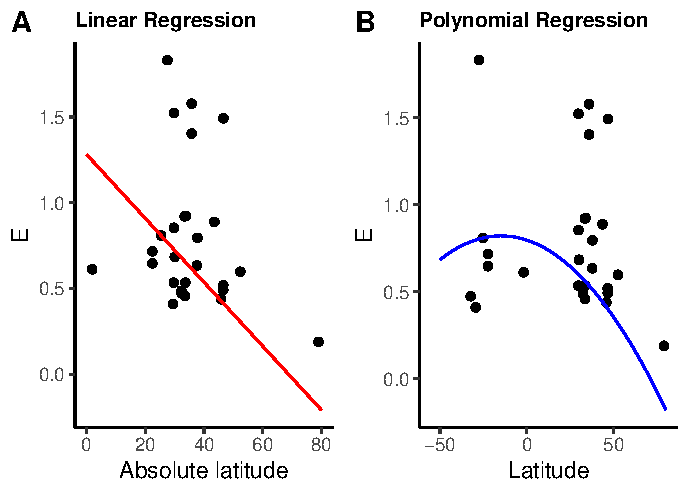
\includegraphics[width=4in]{compare_lat_grid.pdf}
    \caption{\label{fig:5} Model Predictions for (A) linear and (B) polynomial regression of \emph{$E$} in response to varying (A) absolute latitudes and (B) latitudes. The results of this analysis suggest that \emph{E} has a significant relationship with latitude, with $\emph{p}-value < 0.05$.}
\end{figure}

\begin{figure}[!htbp]
    \centering
    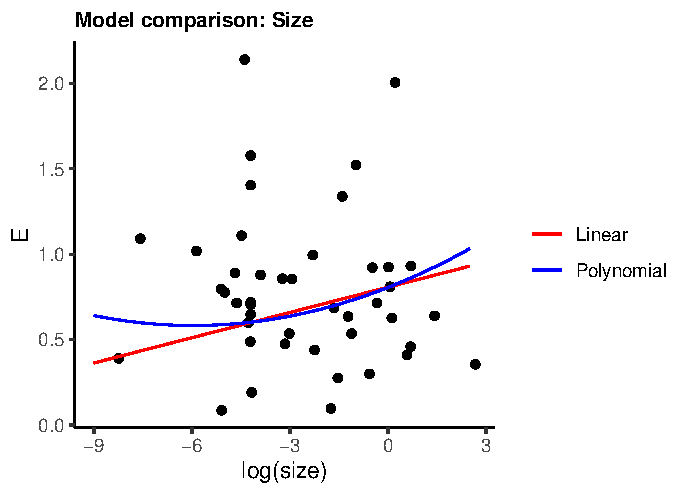
\includegraphics[width=4in]{compare_size.pdf}
    \caption{\label{fig:6} Model Predictions for (A) linear and (B) polynomial regression of $E$ in response to size, measured as the logged mean body mass. The results of this analysis show that \emph{E} has a significant relationship with size, with $\emph{p}-value < 0.05$.}
\end{figure}

\begin{figure}[!htbp]
    \centering
    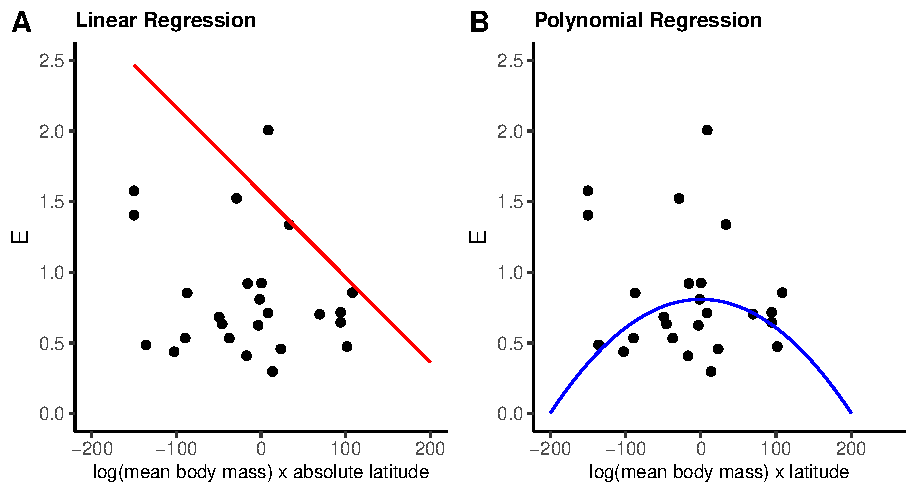
\includegraphics[width=5in]{compare_ls_grid.pdf}
    \caption{\label{fig:7} Model Predictions for (A) linear and (B) polynomial regression of \emph{$E$} in response to the interaction between size and latitude. The results of this analysis suggest that \emph{E} has a significant relationship with the interaction between latitude and body size, with $\emph{p}-value < 0.05$.}
\end{figure}
\clearpage

\section{Discussion}
Thermal sensitivity was estimated for fifty-five species from twenty-eight families by fitting the Sharpe-Schoolfield model to metabolic rate data synthesised from forty studies following an extensive literature review. Phylogenetic heritability ($\lambda$) of $E$ was calculated. No conclusion could be drawn about the heritability of thermal sensitivity from this data, as $\lambda$ estimates show a wide uncertainty around its mean. Therefore, no evidence supporting hypothesis (1) (i.e., that thermal sensitivity is phylogenetically heritable) could be established. The mean value for thermal sensitivity of all fifty-five species in this study was calculated at $\approx$ 0.92 eV, higher than the expected range of 0.6 to 0.7 eV proposed by early metabolic theory (i.e., the Universal Temperature Dependence (UTD)) \citep{gillooly2001effects}.  This finding supports hypothesis (2), that thermal sensitivity of arthropods deviates from the UTD. 
\linebreak

The effect of latitude, body size and the interaction between them on thermal sensitivity was also analysed using linear and polynomial regression models. The model which fit best to the data was the linear regression on latitude, with the overall lowest AIC and BIC values. The regressions on latitude alone produced lower AIC values than the regression on the interaction between both variables. Therefore, the model with the interaction is less informative than the model with only latitude as its predictor. In contrast, the regression on the interaction between size and latitude yielded lower AIC and BIC values than the regression on body size alone, suggesting that the model with only size as a predictor is less informative than the regression on the interaction between size and latitude. The only polynomial model which was included in the AIC and BIC comparisons was for the \emph{$latitude \times size$} regressions. The linear regression model fit the data significantly better than the polynomial model, with an absolute difference of 21.7 for AIC and  20.4 for BIC. These results indicate that the relationship between \emph{E} and (i) latitude, (ii) size and (iii) latitude $\times$ size is linear.
The residuals of these models were used to determine to what degree the relationship between \emph{E} and (i) latitude, (ii) size and (iii) latitude $\times$ size is inherited phylogenetically. Little phylogenetic relationship could be inferred from these values. The interaction between latitude and size predicted by the polynomial regression model yielded the highest phylogenetic signal at 0.7254. All values for $\lambda$ were $<0$, demonstrating deviations from Brownian motion, possibly due to convergence.
\linebreak

\paragraph{Deviation from the Universal Temperature Dependence}\mbox{}\\
Deviations from the UTD may be explained by a number of factors including:
\begin{itemize}
    \item The interaction of multiple factors on trait performance rather than just the single factor of temperature on biochemical kinetics \citep{kontopoulos2020adaptive}. For example, TPCs can be affected by structures which support sites of oxidative phosphorylation (such as membranes and mitochondria) catalysing enzymes and the availability of substrates \citep{delong2018habitat}.
    \item The effect of multiple rate-limiting enzymes rather than a single enzyme \citep{pawar2016real}.
    \item Bias introduced into the analysis by creating “artificial" variance. For example, variation in temperature ranges \citep{pawar2016real}. 
    \item Variation in species, trophic groups and habitats \citep{dell2011systematic,huey2011variation}. 
\end{itemize}
For example, a 2011 study by Dell et al. found that prey tend to have lower $E$ values compared to predators, and exhibit increased trait performance at lower temperatures \citep{dell2011systematic}. Conversely, predators demonstrated higher \emph{E} values. They argued that this may be caused by the “life/dinner" principle, which states that selection is stronger on prey than on predators due a higher consequence of lower trait performance being imposed on the prey species (i.e, death as opposed to losing a meal) \citep{dell2011systematic}. Therefore, a low $E$ value may reflect selection of prey species to possess a high capacity for escape responses across varying temperatures \citep{dell2011systematic,huey2011variation}. Previous analyses which support the existence of a UTD tend to focus on one or relatively few species and, therefore, have restricted generality \citep{huey2011variation}. As this analysis included a broad variation in taxa across different classes, orders and families this may somewhat explain (1) the wide distribution of \emph{$E$} values and (2) a mean \emph{$E$} value higher than the expected range of 0.6-0.7 eV.
\newline 

\paragraph{Limitations and future directions}\mbox{}\\
One limitation of this analysis which may have introduced bias into the results is the relatively small sample size, with only fifty-five species included after filtering. This analysis also may be biased towards certain taxonomic groups within arthropoda, for example, all but four species were insects. There was also a relatively high proportion of ants and crickets. The data were also skewed towards species in the northern hemisphere, with only seven species representing the southern hemisphere. These biases may be due to sampling error. An improvement to this analysis would be to include a larger number of species with adequate representation of each class and equal focus on samples from both the Northern and Southern hemisphere. 
\linebreak
A lack of standardisation of the data on functional traits of arthropods, including their metabolic responses, can lead to a large variation in \emph{E} estimates \citep{pawar2016real}. A good direction of future studies may be to focus on establishing and/or utilizing frameworks for deriving and documenting metabolic data. Although there are useful frameworks for storing metabolic data (for example, the VecTraits framework \citep{samraat_pawar_2016_57356}), a standardised approach to measuring metabolic responses of arthropods to temperature changes has yet to be developed. Such potential frameworks could include a specified range of temperatures, laboratory conditions and a metric for measuring metabolic rate, such as Resting Metabolic Rate.
\linebreak

This analysis may be improved by including another statistic for phylogenetic signal. Blomberg et al.'s \emph{K} \citep{blomberg2003testing} is another measure of phylogenetic heritability. Blomberg's \emph{K} is a scaled value which indicates the strength of phylogenetic heritability as a ratio of the mean squared error of the tip data measured from the corrected mean and mean squared error of the variance–covariance matrix, which is derived from the phylogeny under Brownian Motion \citep{blomberg2003testing,munkemuller2012measure}. In comparison, $\lambda$ measures the similarity of the covariances among species to the covariances expected under Brownian motion, and lies between a value of 0 to 1 \citep{munkemuller2012measure}. It is possible for $\lambda$ to adopt values greater than 1, suggesting that traits of related species are more similar than expected under Brownian motion. However, the upper limit is restricted as off-diagonal elements in the variance–covariance matrix cannot be larger than
the diagonal elements \citep{munkemuller2012measure}. Including another statistical measure for phylogenetic signal and comparing the values may garner more confidence in the results.
\linebreak 

Another addition to this analysis could be to incorporate a Bayesian approach in estimating phylogenetic signal \citep{vrancken2015simultaneously,kontopoulos2020adaptive}. Bayesian inference is a statistical method whereby hypotheses are inferred using prior information (or “priors”). As more information is made available, probability for the hypothesis is also updated. Bayesian methods, therefore, can produce very accurate results; however, results can be more difficult to interpret. A Bayesian approach to this analysis would treat multiple measurements from the same species separately. Therefore, incorporating a Bayesian approach, such as a Markov chain Monte Carlo (MCMC) chain, to this analysis and comparing the results could provide a more robust understanding of the degree to which \emph{E} is phylogenetically heritable.  
\linebreak

\paragraph{Conclusion}\mbox{}\\
In conclusion, the key findings of this study were that (1) \emph{E} does not adhere to the expectations of the Universal Temperature Dependence theory, and was higher than the 0.6 - 0.7 eV range at >0.9 eV. This may be due to a number of factors such as the broad variation of taxa included in this analysis or other underlying mechanistic factors (such as the effect of multiple enzymes or the interaction of multiple factors on trait performance). Another key finding of this study is (2) that latitude, size and the interaction between both significantly affects the thermal performance of arthropods. Latitude seems to have the strongest effect on \emph{E}. This is somewhat expected as temperature is strongly influenced by latitude. A lack of standardised methodology in measuring the response of arthropod metabolism to temperature can introduce a significant amount of error in these estimates. Therefore, future studies may benefit from developing frameworks which to adopt a standardised approach to obtaining and storing this data. A future direction of this analysis would be to incorporate more models (e.g. a MCMC model) and statistical metrics (e.g., \emph{K}) and compare these results to develop a more comprehensive, mechanistic understanding of thermal performance in arthropods.  
\clearpage

\section{Acknowledgements}
I would like to thank my supervisors, Dr. Samraat Pawar, Dr. Dimitris Kontopoulos, Dr. Paul Huxley \&  Dr. Lauren Cator, for all of their guidance, insight and support on this project. I would like to thank Tianle Shao, who helped digitise the data used in this project. I would also like to thank my friends, Jasmine Yang, Juliette Everson, Natalie Nickells, Eamonn Murphy, Kaya Jumbe \& Nicolas Eves, for reading this thesis (or parts of it) and sharing with me their thoughts, as well as giving me some suggestions for some of the methods used in the analysis. 
\newpage
\paragraph{Data and Code Availability Statement:}\mbox{}\\
Github repository: \href{https://github.com/keg121/Project_submission}{\color{blue} \myul[blue] {Click here}} to access repository.

\bibliographystyle{plainnat}
\bibliography{proj}
\end{flushleft}
\end{document}

